\section{The Pinch-Point} \label{sec:pinch}

This is the heart of the derivation. We show that folding distinctions reversibly forces a single number, eight, and
a single structure, the octonions, squeezed from two sides.

\subsection{Folding reversibly is a composition algebra}

To fold one distinction into another is to combine them, a multiplication. To fold \emph{reversibly}, losing nothing,
is to require that the multiplication never destroys information. The precise condition is that the size of a product
is the product of the sizes,
\begin{equation}
  |xy| = |x|\,|y|,
\end{equation}
where $|x|$ is the ordinary length. An algebra with a norm obeying this is a \emph{composition algebra}. The condition
is exactly reversibility, by a short chain. If $|xy| = |x||y|$ and $x, y$ are nonzero, then $|xy| > 0$, so
$xy \neq 0$, so there are no zero divisors, no pair of nonzero elements multiplying to nothing. No zero divisors means
every nonzero element is invertible, a division algebra, with inverse $x^{-1} = \bar{x}/|x|^2$. And invertibility is
reversibility, given $xy$ and $x$ one recovers $y = x^{-1}(xy)$, nothing lost. So the four conditions, the norm
multiplies, no zero divisors, division, reversible, are one and the same. To fold reversibly is to build a composition
algebra.

\subsection{The ceiling, from Hurwitz}

Composition algebras are built by a single repeated move, the Cayley-Dickson doubling (Appendix~\ref{app:tower}),
which from an algebra of dimension $d$ makes one of dimension $2d$. Starting from the integers it gives the tower
\begin{equation}
  \mathbb{Z} \;\to\; \mathbb{C} \;\to\; \mathbb{H} \;\to\; \mathbb{O} \;\to\; \mathbb{S}, \qquad
  1,\;2,\;4,\;8,\;16.
\end{equation}
Each doubling trades away one property. The first loses order ($\mathbb{C}$ has $i^2 = -1$), the second loses
commutativity ($e_1 e_2 \neq e_2 e_1$ in $\mathbb{H}$), the third loses associativity ($(e_1 e_2) e_4 \neq e_1 (e_2 e_4)$
in $\mathbb{O}$). The fourth loses the norm itself.

The reason it loses the norm at exactly the fourth step is a single fact, which we verify by direct computation.

\begin{theorem}[Hurwitz, composition needs associativity]
The Cayley-Dickson double of an algebra $A$ is again a composition algebra if and only if $A$ is associative.
Consequently the composition algebras are exactly $\mathbb{R}$, $\mathbb{C}$, $\mathbb{H}$, $\mathbb{O}$, of dimensions
$1, 2, 4, 8$, and no larger one exists.
\end{theorem}

Walk the tower. $\mathbb{Z}$ (or $\mathbb{R}$) is associative, so its double $\mathbb{C}$ keeps the norm. $\mathbb{C}$
is associative, so $\mathbb{H}$ keeps it. $\mathbb{H}$ is associative, so $\mathbb{O}$ keeps it, even though
$\mathbb{O}$ is itself the first non-associative rung. But $\mathbb{O}$ is not associative, so its double $\mathbb{S}$,
the sedenions, does not keep the norm. We verify the failure concretely, there are two nonzero sedenions with
$(e_1 + e_{10})(e_5 + e_{14}) = 0$, a zero divisor, so $|xy| = 0$ while $|x||y| \neq 0$, and reversibility is gone.
Three doublings succeed because their inputs are associative, the fourth fails because $\mathbb{O}$ is not. Three
doublings give $2^3 = 8$. So eight is the ceiling, and the octonions are the last reversible rung, sitting one step
from the cliff.

\subsection{The floor, from three families}

A particle of matter has spin, a handedness, a left and right the world distinguishes, carried by a \emph{spinor}, a
representation of the rotation cover $\mathrm{Spin}(n)$ that behaves like the square root of a rotation. For almost
every $n$ the spinor and the vector have different dimensions. The exception is $n = 8$. Here $\mathrm{Spin}(8)$ has
three representations all of dimension eight, the vector $8_v$ and two spinors $8_s, 8_c$, and they are cycled by an
order-three symmetry, \emph{triality}. Triality is unique to $\mathrm{Spin}(8)$, because the Dynkin diagram of
$\mathfrak{so}(8) = D_4$ is a three-pointed star, the only one with a threefold symmetry. We verify computationally
that the diagram automorphism group of $D_4$ has order six and contains an order-three element, while every other
$D_n$ has only the order-two flip. The three eight-dimensional representations are the three generations of matter. So
carrying three mirrored families requires triality, which requires dimension eight. Eight is the floor.

\subsection{The meeting}

The two pressures are opposite and they meet at one value.
\begin{equation}
  \text{reversibility}\colon \dim \le 8, \qquad
  \text{three families}\colon \dim \ge 8, \qquad \Longrightarrow \qquad \dim = 8.
\end{equation}

\begin{result}[The octonion is forced]
The unique dimension that is both a composition algebra and large enough to carry triality is eight, and the structure
is the octonions. They are simultaneously the maximal reversible algebra and the minimal triality structure, and they
sit at the last rung before zero divisors appear.
\end{result}

\begin{figure}[ht]
\centering
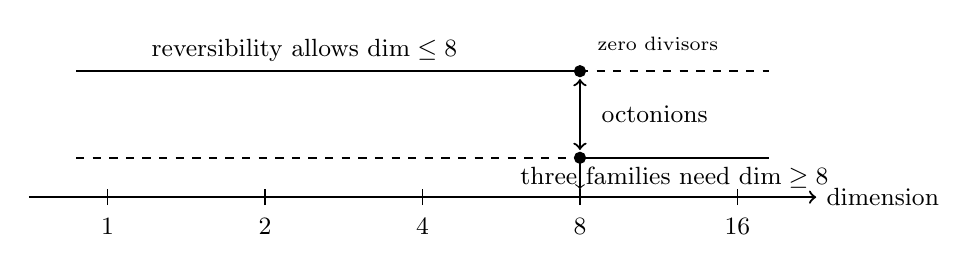
\begin{tikzpicture}[scale=1.0]
  % axis
  \draw[->, thick] (0,0) -- (10,0) node[right] {\small dimension};
  \foreach \x/\d in {1/1, 3/2, 5/4, 7/8, 9/16} {
    \draw (\x,-0.1) -- (\x,0.1);
    \node[below] at (\x,-0.15) {\small \d};
  }
  % ceiling: reversibility, allowed up to 8
  \draw[thick] (0.6,1.6) -- (7,1.6);
  \draw[thick, dashed] (7,1.6) -- (9.4,1.6);
  \node[above] at (3.5,1.6) {\small reversibility allows $\dim \le 8$};
  \node[right] at (7.1,1.95) {\scriptsize zero divisors};
  % floor: triality, needs at least 8
  \draw[thick] (7,0.5) -- (9.4,0.5);
  \draw[thick, dashed] (0.6,0.5) -- (7,0.5);
  \node[below] at (8.2,0.5) {\small three families need $\dim \ge 8$};
  % the pinch at 8
  \filldraw (7,1.6) circle (2pt);
  \filldraw (7,0.5) circle (2pt);
  \draw[<->, thick] (7,1.5) -- (7,0.6);
  \node[right] at (7.15,1.05) {\small octonions};
  \draw[->] (7,0.45) -- (7,0.1);
\end{tikzpicture}
\caption{The pinch-point. Reversibility caps the dimension at eight from above (Hurwitz). Three mirrored families
floor it at eight from below (triality). The two meet only at eight, the octonions, the last rung before zero
divisors break reversibility.}
\label{fig:pinch}
\end{figure}

The octonions are not chosen, not tuned. They are squeezed into being. A world of dimension four, the quaternions,
would be reversible but could carry no triality, no three families. A world of dimension sixteen could carry families
but would not be reversible, it has zero divisors. Only eight is both, and eight is the edge. This is why the result
feels finely poised. It is finely poised. The world is built at the maximal reversible size, one step from the cliff
where folding stops being reversible at all. The rest of this paper reads off what the octonion then builds.
